%%%%%%%%%%%%%%%%%%%%%%%%%%%%%%%%%%%%%%%%%%%%%%%%%%%%%%%%%%%%%%%%%%%%
%% %%	Posterdown PDF class for LaTeX files	 08-JAN-2019
%% %%	For any information please send an e-mail to:
%% %%		brentthonre18@gmail.com (Brent Thorne)
%% %%
%% %%	Initial class provided by:
%% %%		Brent Thorne
%% %% Contributors: Shea Connell (SC)
%%%%%%%%%%%%%%%%%%%%%%%%%%%%%%%%%%%%%%%%%%%%%%%%%%%%%%%%%%%%%%%%%%%%

\documentclass[article,30pt,extrafontsizes]{memoir}

%utf-8 seems to be important
\RequirePackage[utf8]{inputenc}
\RequirePackage[T1]{fontenc}
\RequirePackage{lmodern}
\RequirePackage{multicol}
\RequirePackage{graphicx}
\RequirePackage{lipsum}
\RequirePackage{blindtext}
\RequirePackage[svgnames,table]{xcolor}
\RequirePackage{tikz}
\RequirePackage[framemethod=tikz]{mdframed}
\RequirePackage{color}
\RequirePackage{geometry}
\RequirePackage{adjmulticol}
\RequirePackage[skins,most,listings,skins]{tcolorbox}

%For kable extra package :)
\RequirePackage{booktabs}
\RequirePackage{longtable}
\RequirePackage{array}
\RequirePackage{multirow}
\RequirePackage{wrapfig}
\RequirePackage{float}
\RequirePackage{colortbl}
\RequirePackage{pdflscape}
\RequirePackage{pagecolor}
\RequirePackage{tabu}
\RequirePackage{threeparttable}
\RequirePackage{threeparttablex}
\RequirePackage[normalem]{ulem}
\RequirePackage{makecell}
\RequirePackage{wrapfig}

%rof hyperrefs
\RequirePackage{hyperref}
\hypersetup{
    colorlinks=true,
    linkcolor=linkcol,
    citecolor=citecol,
    filecolor=linkcol,
    urlcolor=urlcol,
}
%For figure and table placement
\RequirePackage{float}
\floatplacement{figure}{H}
\floatplacement{table}{H}

%%%%%%%%% COLOURS %%%%%%%%
%Fill/ Line Colours
\definecolor{titleboxbgcol}{HTML}{008080}
\definecolor{titleboxbordercol}{HTML}{0b4545}
\definecolor{columnlinecol}{HTML}{008080}
\definecolor{bodybgcol}{HTML}{ffffff}
\definecolor{sectitlebgcol}{HTML}{0b4545}
\definecolor{sectitlebordercol}{HTML}{0b4545}
% Text Colours
\definecolor{titletextcol}{HTML}{ffffff}
\definecolor{authortextcol}{HTML}{0b4545}
\definecolor{affiliationtextcol}{HTML}{FFFFFF}
\definecolor{sectitletextcol}{HTML}{ffffff}
\definecolor{bodytextcol}{HTML}{000000}
\definecolor{footnotetextcol}{HTML}{ffffff}
\definecolor{citecol}{HTML}{CC0000}
\definecolor{urlcol}{HTML}{008080}
\definecolor{linkcol}{HTML}{008080}


%Memoir spacing options
%spacing between figure/ table and caption
\setlength{\abovecaptionskip}{0.4in}
\setlength{\belowcaptionskip}{0.2in}
\captionnamefont{\footnotesize\sffamily\bfseries}
\captiontitlefont{\footnotesize\sffamily}

%define column options
\setlength{\columnseprule}{0pt}
\def\columnseprulecolor{\color{columnlinecol}}

%define section title features
\setsubsubsecheadstyle{\small\color{sectitletextcol}\textbf}% Set \section style
\setsecnumformat{}
\def\sectionmark#1{\markboth{#1}{#1}}

%%%%%%%%%%%% TCOLORBOXES TO THE RESCUE %%%%%%%%%%%%%%%%%%%%
%Title Box
\newtcolorbox{topbox}{
enhanced,
colback=titleboxbgcol,
colframe=titleboxbordercol,
halign=center,
boxrule=1cm,
sharp corners=all,
 overlay={
    \node[anchor=south west]
      at ([xshift=1in,yshift=1in]frame.south west)
       {
\includegraphics[width=3in]{Figures/posterdownlogo}};
    \node[anchor=south east]
      at ([xshift=-1in,yshift=1in]frame.south east)
       {
\includegraphics[width=3in]{Figures/posterdownlogo}};}

}
%Body Section Title Box
\newtcolorbox{myboxstuff}[1][]{
code={\parindent=0em},
colframe=sectitlebordercol,
nobeforeafter,
left skip=0pt,
valign=center,
halign=center,
fontupper=\Large\bfseries,
colupper=sectitletextcol,
boxrule=2mm,
colback=sectitlebgcol,
sharp corners=uphill, #1}
\newcommand{\mybox}[1]{%
\begin{myboxstuff}
\strut #1
\end{myboxstuff}%
}
\makeheadstyles{MyBox}{
    \setsecheadstyle{\mybox}
}
\headstyles{MyBox}\makepagestyle{MyBox}
%-----------------------------------------------------
%Make sure that the page is empty of any preset items from memoir
\thispagestyle{empty}

%biblatex options
\RequirePackage[sorting=none,backend=biber]{biblatex}
\renewcommand*{\bibfont}{\small} %% SC
\bibliography{MyLibrary}
\defbibheading{bibliography}[\bibname]{%
\setlength\bibitemsep{0.8\itemsep} %% SC
\section*{#1}%
\markboth{#1}{#1}}
\AtBeginDocument{%
  \renewcommand{\bibname}{References}
}

%Remove section numbering & set 2nd level header as first level
%to avoid the automatic new page generated from memoir chapter
%formatting
\counterwithout{section}{chapter}
\makechapterstyle{mydefault}{
\addtocounter{secnumdepth}{2}
\setsecheadstyle{\mybox}
\setsubsecheadstyle{\itshape}
\setsubsubsecheadstyle{\itshape}
}

%set the chapterstyle
\chapterstyle{mydefault}

%define column spacing
\setlength\columnsep{0.5in}

%spacing params
\setlength\parindent{0em}
\setlength\parskip{0em}
\setlength\hangparas{0}

%spacing after section head title
\setaftersecskip{0em}
\setbeforesecskip{1.5em}
\setlength\textfloatsep{0in}
\setlength\floatsep{0in}
\setlength\intextsep{0in}

\setstocksize{32in}{40in}
\settrimmedsize{\stockheight}{\stockwidth}{*}
\settypeblocksize{32in}{40in}{*}
\setlrmargins{*}{*}{1}
\setulmarginsandblock{2.5cm}{*}{*}
\setmarginnotes{0em}{0cm}{0cm}
\setlength{\footskip}{0cm}
\setlength{\footnotesep}{0cm}
\setlength{\headheight}{0pt}
\setlength{\headsep}{0pt}
\setlength{\trimtop}{0pt}
\setlength{\trimedge}{0pt}
\setlength{\uppermargin}{0pt}
\checkandfixthelayout

%Footnote to white
\RequirePackage{footmisc}
\def\footnotelayout{\centering\color{footnotetextcol}}

% see https://stackoverflow.com/a/47122900
\usepackage{color}
\usepackage{fancyvrb}
\newcommand{\VerbBar}{|}
\newcommand{\VERB}{\Verb[commandchars=\\\{\}]}
\DefineVerbatimEnvironment{Highlighting}{Verbatim}{commandchars=\\\{\}}
% Add ',fontsize=\small' for more characters per line
\usepackage{framed}
\definecolor{shadecolor}{RGB}{248,248,248}
\newenvironment{Shaded}{\begin{snugshade}}{\end{snugshade}}
\newcommand{\AlertTok}[1]{\textcolor[rgb]{0.94,0.16,0.16}{#1}}
\newcommand{\AnnotationTok}[1]{\textcolor[rgb]{0.56,0.35,0.01}{\textbf{\textit{#1}}}}
\newcommand{\AttributeTok}[1]{\textcolor[rgb]{0.77,0.63,0.00}{#1}}
\newcommand{\BaseNTok}[1]{\textcolor[rgb]{0.00,0.00,0.81}{#1}}
\newcommand{\BuiltInTok}[1]{#1}
\newcommand{\CharTok}[1]{\textcolor[rgb]{0.31,0.60,0.02}{#1}}
\newcommand{\CommentTok}[1]{\textcolor[rgb]{0.56,0.35,0.01}{\textit{#1}}}
\newcommand{\CommentVarTok}[1]{\textcolor[rgb]{0.56,0.35,0.01}{\textbf{\textit{#1}}}}
\newcommand{\ConstantTok}[1]{\textcolor[rgb]{0.00,0.00,0.00}{#1}}
\newcommand{\ControlFlowTok}[1]{\textcolor[rgb]{0.13,0.29,0.53}{\textbf{#1}}}
\newcommand{\DataTypeTok}[1]{\textcolor[rgb]{0.13,0.29,0.53}{#1}}
\newcommand{\DecValTok}[1]{\textcolor[rgb]{0.00,0.00,0.81}{#1}}
\newcommand{\DocumentationTok}[1]{\textcolor[rgb]{0.56,0.35,0.01}{\textbf{\textit{#1}}}}
\newcommand{\ErrorTok}[1]{\textcolor[rgb]{0.64,0.00,0.00}{\textbf{#1}}}
\newcommand{\ExtensionTok}[1]{#1}
\newcommand{\FloatTok}[1]{\textcolor[rgb]{0.00,0.00,0.81}{#1}}
\newcommand{\FunctionTok}[1]{\textcolor[rgb]{0.00,0.00,0.00}{#1}}
\newcommand{\ImportTok}[1]{#1}
\newcommand{\InformationTok}[1]{\textcolor[rgb]{0.56,0.35,0.01}{\textbf{\textit{#1}}}}
\newcommand{\KeywordTok}[1]{\textcolor[rgb]{0.13,0.29,0.53}{\textbf{#1}}}
\newcommand{\NormalTok}[1]{#1}
\newcommand{\OperatorTok}[1]{\textcolor[rgb]{0.81,0.36,0.00}{\textbf{#1}}}
\newcommand{\OtherTok}[1]{\textcolor[rgb]{0.56,0.35,0.01}{#1}}
\newcommand{\PreprocessorTok}[1]{\textcolor[rgb]{0.56,0.35,0.01}{\textit{#1}}}
\newcommand{\RegionMarkerTok}[1]{#1}
\newcommand{\SpecialCharTok}[1]{\textcolor[rgb]{0.00,0.00,0.00}{#1}}
\newcommand{\SpecialStringTok}[1]{\textcolor[rgb]{0.31,0.60,0.02}{#1}}
\newcommand{\StringTok}[1]{\textcolor[rgb]{0.31,0.60,0.02}{#1}}
\newcommand{\VariableTok}[1]{\textcolor[rgb]{0.00,0.00,0.00}{#1}}
\newcommand{\VerbatimStringTok}[1]{\textcolor[rgb]{0.31,0.60,0.02}{#1}}
\newcommand{\WarningTok}[1]{\textcolor[rgb]{0.56,0.35,0.01}{\textbf{\textit{#1}}}}

% choose font family
\RequirePackage{palatino}

% define the BODYBGCOL
\newpagecolor{bodybgcol}

%sets footnote to be white hopefully
\renewcommand\footnoterule{}
\renewcommand{\thempfootnote}{\footnotesize\color{footnotetextcol}{\arabic{mpfootnote}}}

%include arbitrary input from header-includes field

%-------------- Begin Document -------------------%
\begin{document}

%-------------- Title Box Start ------------------%
%tcolorbox allows for pictures hopefully
\begin{topbox}
  \color{titletextcol}
  \vspace{0.5in}
  \Huge{\fontfamily{phv}\selectfont Parents and children in diverse languages
structure their utterances to support efficient communication}  \\[0.3in]  %% SC
  \color{authortextcol} \Large{Josef Klafka Daniel Yurovsky} \\[0.2in] %% SC
  \color{affiliationtextcol} \large{\textsuperscript{1}Department of Psychology, University of Chicago} %% SC
  \vspace{1cm}
\end{topbox}
%--------------- Title Box End -------------------%
%----------------- Body Start --------------------%
% Begin body of poster
\begin{adjmulticols*}{2}{0.5in}{0.5in}
\normalsize{  %% SC
\color{bodytextcol}
\hypertarget{introduction}{%
\section{Introduction}\label{introduction}}

Welcome to \texttt{posterdown} ! This is my attempt to provide a
semi-smooth workflow for those who wish to take their R Markdown skills
to the conference world. Most features from R Markdown are available in
this package such as Markdown section notation, figure captioning, and
even citations like this one \autocite{rmarkdown}. The rest of this
example poster will show how you can insert typical conference poster
features into your own document.

\hypertarget{objectives}{%
\subsection{Objectives}\label{objectives}}

\begin{enumerate}
\def\labelenumi{\arabic{enumi}.}
\tightlist
\item
  Easy to use reproducible poster design.
\item
  Integration with R Markdown.
\item
  Easy transition from \texttt{posterdown} to \texttt{thesisdown} or
  \texttt{rticles} \autocites{rticles}{thesisdown}.
\end{enumerate}

\hypertarget{methods}{%
\section{Methods}\label{methods}}

This package uses the same workflow approach as the R Markdown you know
and love. Basically it goes from RMarkdown \textgreater{} Knitr
\textgreater{} Markdown \textgreater{} Pandoc \textgreater{} HTML/CSS
\textgreater{} PDF. You can even use the bibliography the same way
\autocite{turnerControlsWaterBalance2014}.

\hypertarget{random-text}{%
\subsection{Random text}\label{random-text}}

Lorem ipsum dolor sit amet, consectetur adipiscing elit. Aliquam
placerat augue at velit tincidunt semper. Donec elementum porta posuere.
Nullam interdum, odio at tincidunt feugiat, turpis nisi blandit eros, eu
posuere risus felis non quam. Nam eget lorem odio. Duis et aliquet orci.
Phasellus nec viverra est. Praesent odio orci, mattis vel mauris nec,
consectetur fermentum mauris. Etiam eu hendrerit tortor. Donec mi
tellus, efficitur et porttitor eu, auctor eu tellus. Quisque faucibus
vestibulum sapien vel lacinia. Ut auctor lorem non interdum blandit.

\hypertarget{results}{%
\section{Results}\label{results}}

Usually you want to have a nice table displaying some important results
that you have calculated. In \texttt{posterdown} this is as easy as
using the \texttt{kable} table formatting you are probably use to as per
typical R Markdown formatting. I suggesting checking out the
\texttt{kableExtra} package and its in depth documentation on
customizing these tables found
\href{https://haozhu233.github.io/kableExtra/awesome_table_in_pdf.pdf}{here}
\autocite{kableExtra2019}. You can reference tables like so: Table
@ref(tab:mytable).

Table caption.

Sepal.Length

Sepal.Width

Petal.Length

Petal.Width

5.1

3.5

1.4

0.2

4.9

3.0

1.4

0.2

4.7

3.2

1.3

0.2

4.6

3.1

1.5

0.2

5.0

3.6

1.4

0.2

Or with figures: Figure @ref(fig:standard-plot).

\begin{Shaded}
\begin{Highlighting}[]
\KeywordTok{plot}\NormalTok{(mtcars[}\DecValTok{1}\OperatorTok{:}\DecValTok{2}\NormalTok{])}
\end{Highlighting}
\end{Shaded}

\begin{figure}

{\centering 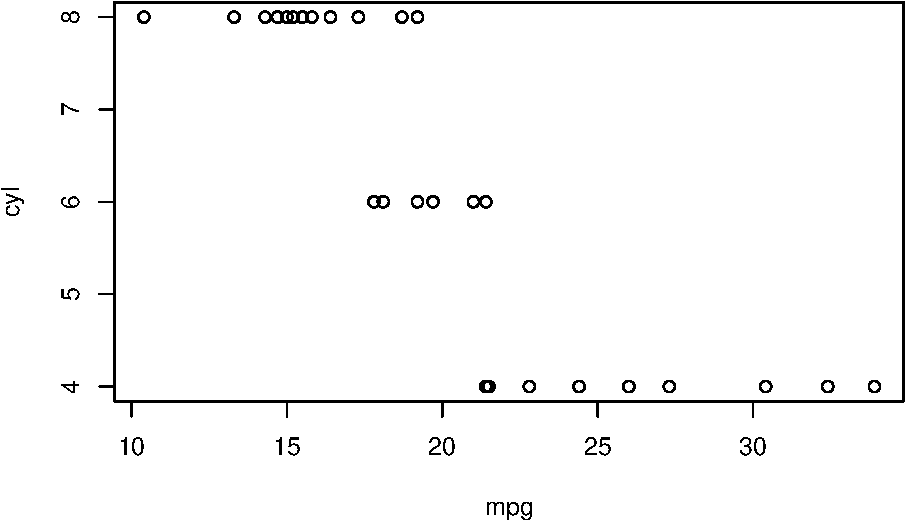
\includegraphics[width=0.8\linewidth]{MacWhinney_Poster_files/figure-latex/standard-plot-1} 

}

\caption{Great figure!}\label{fig:standard-plot}
\end{figure}

\hypertarget{next-steps-more-random-text}{%
\section{Next Steps: More random
text}\label{next-steps-more-random-text}}

Aliquam sed faucibus risus, quis efficitur erat. Vestibulum semper
mauris quis tempus eleifend. Aliquam sagittis dictum ipsum, quis viverra
ligula eleifend ut. Curabitur sagittis vitae arcu eget faucibus. In non
elementum felis. Duis et aliquam nunc. Nunc pulvinar sapien nunc, vel
pretium nisi efficitur in. Fusce fringilla maximus leo et maximus. Fusce
at ligula laoreet, iaculis mi at, auctor odio. Praesent sed elementum
justo. Aenean consectetur risus rhoncus tincidunt efficitur. Praesent
dictum mauris at diam maximus maximus \autocite{thorneposterdown2019}.

\hypertarget{conclusion}{%
\section{Conclusion}\label{conclusion}}

Try \texttt{posterdown} out! Hopefully you like it!

\hypertarget{references}{%
\section{References}\label{references}}

\printbibliography
}
\end{adjmulticols*}
%------------------ Body End ---------------------%
%end the poster
\end{document}

